%%%%%%%%%%%%%%%%%%%%%%%%%%%%%%%%
\section{Energy Harvesting for Electric Vehicles} \label{sec:harvesting}
%%%%%%%%%%%%%%%%%%%%%%%%%%%%%%%%

Energy harvesting refers to harnessing energy from the environment or other sources (e.g. solar, thermal energy, friction etc.) and converting it to electrical energy.
In electric vehicles, energy harvesting works as an important energy resource, which can save a lot of electric energy and thus can extend the range of electric vehicles with the same charging time.
Nowadays, a lot of electric vehicles are powered by harvested energy or hybrid energy including harvested energy, such as solar energy, wind energy, and energies brought by vehicle shock/vibration and brakes.
In the following, we survey different energy harvesting techniques in electric vehicles and summarize the research work on different sources of harvested energies on electric vehicles.

%%%%%%%%%%%%%%%%%%%%%%%%%%%%%%%%
\subsection{Energy Sources}

\subsubsection{Solar}

As one of the most important renewable energy sources, solar energy is positioned to reduce the use of natural gas and coal for electricity generation and to provide electricity for the plug-in electric vehicle market \cite{JX_fthenakis2009technical}.
Abundant sunlight makes it perfect to be used as an alternative energy on electric hybrid vehicles \cite{JX_singh2012study,JX_bourgeois2015harvesting}.
The annual potential of solar energy is several times larger than the total energy consumption in the world.

The most common mechanism to harvest solar energy is directly converting the light into direct current electricity via the photovoltaic effect.
Fig.~\ref{fig:JX_circuit} shows the system circuit of a photovoltaic (PV) powered electric vehicle, which consists of a PV array and peripheral charging regulation circuitry \cite{JX_wang2012dynamic}\cite{JX_kim2014fast}.
A PV array consists of a number of series-connected PV cell groups where each PV group consists of (potentially a different number of) PV cells connected in parallel.
The PV array are mounted on the roof panel, engine hood, trunk, and door panels of the electric vehicles.
Conventional electric vehicles are equipped with battery packs as the energy storage system, connected to the traction motor via the generator charger.
The PV-powered electric vehicle also has an add-on PV system that consists of a PV array and a PV charger connecting the PV array to battery packs.
The generator charger and PV charger can simultaneously charge battery packs.
Maximum power point tracking (MPPT) techniques are integrated with the PV charger, which are employed in photovoltaic systems to make full utilization of PV array for large output power \cite{JX_liu2008variable,JX_arsie2006hybrid,JX_ma2009research}.
Therefore, the PV charger can set the optimal operating point for the PV array.
There are three main issues for solar energy harvesting.

\begin{figure}
\centering
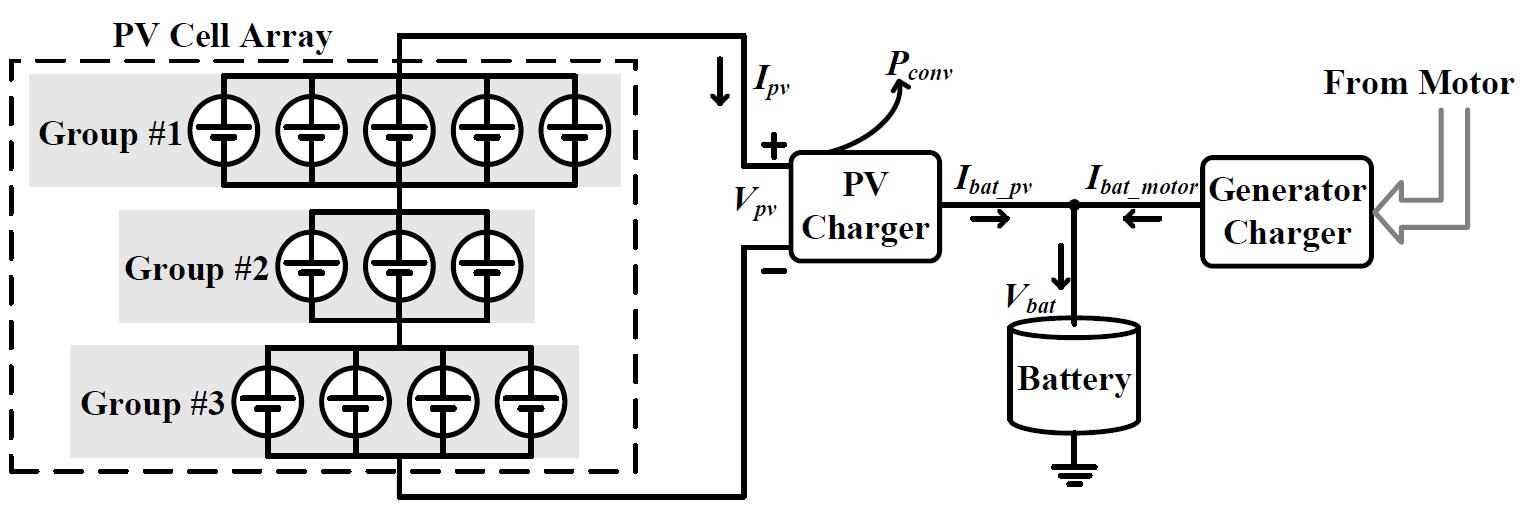
\includegraphics[width=1.0\hsize]{Figures/Jason_Xue/JX_circuit.jpg}
\caption{Circuit of a PV system on a electric vehicle~\cite{JX_wang2012dynamic}.}
\label{fig:JX_circuit}
\end{figure}      


First, since the PV cell array is installed on different parts of a vehicle body such as the engine hood, door panels, and the roof panel, and the system suffers from non-uniformity of the solar irradiance and partial shading phenomenon.
Partial shading of PV arrays is one of the hottest problem in the field of solar photovoltaic.
It exhibits multiple peaks in the PV and thus reduces the overall output power \cite{JX_rajan2017solar}.
As a result, the modules have to be reconfigured to get a maximum power output.
Many previous work \cite{JX_wang2012dynamic,JX_kim2014fast,JX_storey2014optimized,JX_arsie2006optimal} presented dynamic PV array reconfiguration techniques to produce the near-optimal reconfiguration of the PV array on the electric vehicle.
For these work, the goal is to maximize the PV system output power under any solar irradiance and temperature distribution on the PV array.
A model is developed in \cite{JX_vicente2015photovoltaic} to describe the effects of solar panels area and position, vehicle dimensions and propulsion system components on vehicle performance, and further exploited it for optimization.


Second, the difference in energy demand for DC motor impacts the lifetime of the battery.
When the car is decelerating, energy demand for the DC motor is very less and voltage drop of battery is negligible.
However, when the car is accelerating, climbing slope or starting, the motor will cause a large current impulse, which may lead to large voltage drop on the battery.
This will affect power quality of DC source and lifetime of battery.
In order to avoid this, \cite{JX_vincent2013advanced,JX_hopkins2015high,JX_agrawal2016multi} proposed to employs a super capacitor.
When the car is decelerating, super capacitor will charge up to its rated voltage.
Multi-port converter interfacing a photovoltaic array, battery and a DC load is proposed.
It is composed of a two uni-directional DC port for interfacing photovoltaic array and DC load, and a bi-directional DC port for interfacing battery.
The capacitor which is connected to the lead acid battery will charge at off peak hours and discharge during the acceleration time of the car.
The control strategy of bi-directional converter is proposed, which operates at three operation modes: charge battery, discharge battery, and shut-down.
The advantage is better protection and more efficient control on charge/discharge of the battery.

The third issue of solar vehicle is to achieve the the routing request in bounded time \cite{JX_chen2013green,JX_aqeel2016optimized,JX_elizabeth2016velocity,JX_lv2016speed}.
Particle swarm optimization is adopted to make sure that the vehicle reaches the destination within the user defined delay \cite{JX_chen2013green}.
The energy consumption ratio in \cite{JX_aqeel2016optimized} is introduced to measure the efficiency of the solar vehicle which is denoted as arrival ratio divided by energy consumption. The aim is to achieve a high energy consumption ratio for the time-bounded routing request.
The work \cite{JX_elizabeth2016velocity} proposed to optimally plan the speed on different road segments and thus balancing energy harvesting and consumption
With the consideration of the solar illumination and the traffic flow, a suitable speed is predicted for the solar vehicle to have the minimum energy using in moving.

In addition, by using nano-materials the incident radiation can be increased by 9 times \cite{JX_abdin2013solar} while the efficiency of the solar collector is 10\% higher compared to that of a conventional flat plate solar collector.

\textcolor{red}{The amount of power generated by PVs is maximum 200 W per square meter under 1 kW input solar power. On the other hands, EV power consumption is average 16 kW when Tesla Model S drives at 55 mph. Therefore, a simple calculation shows that PV power generation is way shorter than the EV power consumption. However, PV energy harvesting is still useful when the vehicle is parked for hours. PV panels on the EV can harvest  driving energy for significant if the EV is driven for commute in the morning and evening while it is parked at the non-covered parking lot during the whole daytime.}

%\subsubsection{Wind energy}

%Wind energy, similar to solar energy is a common energy source which is harvested and transformed to electricity in many areas.
%For (electric) vehicles, when it is moving, wind will cause a drag force which is opposite to the direction of the propulsion of the vehicle.
%Now if these stream generated by the interaction of the wind and vehicle is captured in such a way that it would not impose an additional drag at the direction of propulsion of the vehicle, some of the energy can be recovered and fed back to the battery by means of conventional energy conversion processes.
%Placing a wind turbine, which can be mounted on the body structure of the vehicle can serve the purpose to generate electricity \cite{JX_Moshfegh,JX_7006196}. %[149] India paper for BUS. [177] Wired reference.

%One major challenge of harvesting wind energy through wind turbines is that normally wind speed varies significantly, which causes voltage and power fluctuation problems at the load side \cite{JX_6183172}.
%When the wind speed is high, the peak power might bring damage to the electric system.
%Also, the extra power can be wasted during the high-speed period.
%The system thus should be able to efficiently store the energy generated by wind turbines for future use when no wind is available \cite{JX_KHAN2005421}. % no onboard windmill on EV
%To achieve this, one way is to appropriately utilize power converters and control strategies to inject proper power to grid \cite{JX_8077284,JX_7925346,JX_1304613}. % [151] no onboard windmill on EV  [178] Mixing stationary and onboard windmill, low quality paper  [179] Not relevant (thermal)
%Another conventional method is to store wind energy after appropriate conversion in the form of hydrogen which will be converted to electrical energy via fuel cells \cite{JX_ONAR2006707}. % [180]
%In \cite{JX_DEBATTISTA2006478}, power conditioning for a wind-hydrogen energy system has been reported. %[144] no onboard windmill on EV
%In \cite{JX_BECHRAKIS200646}, a simulation and operational assessment is investigated for a small autonomous wind-hydrogen energy system.
%[145] no onboard windmill on EV

%Normally, wind energy is not the only harvest energy source in electric vehicles.
%It is often combined with solar energy together to support the process of electric vehicles \cite{JX_8077284,JX_7006196,JX_4762597}.
% [149] India paper for BUS [179] Not relevant (thermal) [185] no onboard EV (not relevant)

\subsubsection{Regenerative shock absorbers}

When an electric vehicles move in the road, the suspension power of the conventional shock absorbers are normally dissipated through friction and heat.
However, these wasted energy in a vehicle's shock absorber can be collected and converted to an alternative electric energy through energy regenerative shock absorber, as shown in Fig.~\ref{fig:JX_shock}.

\begin{figure}
\centering
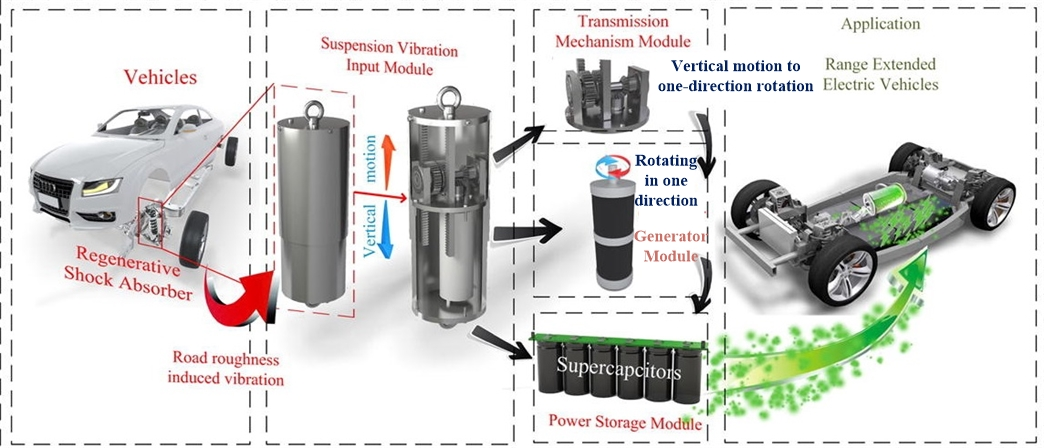
\includegraphics[width=1.0\hsize]{Figures/Jason_Xue/JX_shock.jpg}
\caption{Regenerative shock energy converted into electricity~\cite{JX_ZHANG2016177}.}
\label{fig:JX_shock}
\end{figure}      

Fundamental research has examined and analyzed the feasibility of harvesting energy from the shock absorber since the 1980s \cite{JX_ref1}.
The regenerative shock absorber was proposed to harvest the kinetic energy dissipated by the suspension vibration in the shock absorber.
In \cite{JX_ref1}, the authors described and analyzed how energy lost in a car shock absorber corresponding to different vehicles' speed and road roughness.
Recent studies further uncovered the potential of energy harvesting from the shock absorber \cite{JX_JOUR,JX_HUANG201516}.
The work \cite{JX_JOUR} made a significant improvement in the energy harvesting and ride comfort of regenerative vehicle suspensions over existing techniques.
The authors presented a regenerative shock absorber and estimated a power range of 100$\sim$400 W at 100 km/h depending on the road profile.
In \cite{JX_HUANG201516} the authors proposed an analytical methodology based on ground tire interface analysis and ride comfort cost function for an energy-regenerative suspension design.
This research work aimed to achieve optimal performance and ride comfort and derive the closed-form solutions of the performance metrics for an energy-regenerative suspension.
Among these initial theoretic studies, the shock absorber was transformed into an energy harvesting device from an energy dissipating device.
Possible noise and heat in the conventional working progress are eliminated, which is environmentally friendly and lifetime extending.

With respect to long-term evolution and development, regenerative shock absorbers can be classified into three categories based on their working principles: electromagnetic, hydraulic and mechanical designs.

The first category directly uses an electromagnetic method to generate the electric power.
The methods include linear \cite{JX_0964-1726-19-4-045003,JX_5737802,JX_ZHANG20121124,JX_2619394820151001,JX_XIE2015385} and rotary schemes \cite{JX_6063995,JX_6023317}.
A linear electromagnetic regenerative shock absorber converts the kinetic energy of vertical oscillations into electricity by electromagnetic induction.
The structure of linear schemes is simple and kinetic energy is converted directly.
Unlike normal linear movement damper, rotary damper rotates by the upper arm of suspension when tire move up and down.
This structure has high efficiency which can reach 90\% for both driving and back driving but needs to change suspension structure largely which in turn will have influence on the handling and stability performance.

For the second category, hydraulic regenerative shock absorbers can harvest the vibration energy and convert this energy into electricity by employing oscillatory motion to drive the power generator.
They utilized commercial DC/AC motors as generators and focused on various methods to drive these generators.
A number of studies reformed the existing hydraulic shock absorber and utilized the oil in the shock absorber to flow into a side oil circuit \cite{JX_doi,JX_ZHANG2015485}.
They normally use the flowing fluid to drive a hydraulic motor, which is connected in parallel to a DC/AC generator.
Check valves are also used to ensure unidirectional fluid flow and unidirectional rotation of the hydraulic motor.

The third category is mechanical design, which is developed rapidly because of a greater efficiency and average power.
In previous studies \cite{JX_6063995,JX_pub1643510,JX_6587850,JX_7057652}, ball screws have been used for the transmission of regenerative shock absorbers for the sake of good stiffness and transmitting efficiency.
An energy regenerative suspension is designed and improved using an algebraic screw linkage in \cite{JX_6587850,JX_7057652}.
A hexagon linkage was used in the initial design, and a two-leg linkage was presented in latter schemes.
The work \cite{JX_Gupta2006} compared different electromagnetic shock absorbers and found that rotary schemes had large power compared with the linear schemes in bench tests.
The results also indicated that rack and gears have the potential to drive a larger DC/AC motor to achieve greater power density.
In \cite{JX_5545646}, the authors analyzed and modeled an equivalent circuit for an electromagnetic regenerative shock absorber using a rack and gears.
This model assisted the evaluation and optimization of the rack-and-gears schemes. Rack-and-gears regenerative shock absorbers based on a mechanical design were rapidly developed because of their high efficiency and average power \cite{JX_6399623,JX_0964}.

\subsubsection{Regenerative braking}

Regenerative braking is that the kinetic energy from a moving car generates electricity back to the battery when a vehicle is in coasting and braking modes as shown in Fig.~\ref{fig:JX_break}.
With regenerative braking technique, it is shown that electric vehicles can increase the driving distance up to 15\% with respect to electric vehicles without the regenerative braking system.

\begin{figure}
\centering
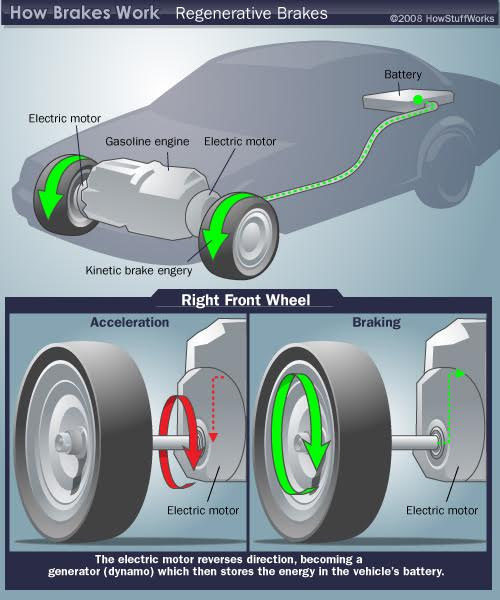
\includegraphics[width=1.0\hsize]{Figures/Jason_Xue/JX_brake.jpg}
\caption{Regenerative brakes~\cite{JX_regen_fig}.}
\label{fig:JX_break}
\end{figure}      

According to different ways to capture the energy generated by regenerative braking, the-state-of-the-art regenerative braking systems can be clarified into the following four types.
First, the electricity generated is stored directly into batteries.
Unfortunately, due to frequent charging, the lifetime of batteries will be decreased \cite{JX_4450599,JX_4677669}.
Second, instead of directly charging to battery, ultracapacitors/supercapacitors are used to store the energy from regenerative braking \cite{JX_5764539,JX_5446335}
Besides, ultracapacitors are the options with higher power densities compared to batteries.
The above two kinds of systems can capture and return around 50\% of the energy lost in braking \cite{JX_DATE,JX_Tie2013}.

Third, the break energy can be stored by hydraulic motors into a small canister through compressed air. When you hit the brakes, this system engages a pump which forces compressed air into a tank.
This converts the mechanical energy of motion into elastic energy in the gas.
These systems can capture and return around 70\% of the energy lost in braking \cite{JX_2002013128,JX_2008valents}.

The last way is that, energy can also be stored in Flywheel energy system (FES) as rotating energy.
When you hit the brakes, this system transfers the mechanical energy of motion into electricity, which is then used to speed up the flywheel \cite{JX_5472647,JX_5686984,JX_993788}.
These systems can capture and return around 70\% of the energy lost in braking \cite{JX_DATE}.


